Lagrange multipliers:


$\min \mathcal{L}(\vec{X}, \vec{\lambda}) = f(\vec{X}) +\vec{\lambda}^T \vec{g}$

necessary condition:
$$\vec{\nabla} \mathcal{L}  =  \begin{bmatrix}
	 \vec{\nabla}_{\vec{X}} \mathcal{L} \\[6pt]
	 \vec{\nabla}_{\vec{\lambda}} \mathcal{L}
\end{bmatrix} = \begin{bmatrix}
\dfrac{\partial \mathcal{L}}{\partial \vec{X}} \\[10pt]
\dfrac{\partial \mathcal{L}}{\partial \vec{\lambda}}
\end{bmatrix} = \vec{0}$$
$f(\vec{X}) = x^2 + y^2 + z^2, \quad  g(\vec{X}) = \sin(x) + \cos(y) - z = 0$
$$\min \mathcal{L}(\vec{X}, \vec{\lambda}) = x^2 + y^2 + z^2 + \lambda (\sin(x) + \cos(y) - z)$$
$$\vec{\nabla} \mathcal{L} = \begin{bmatrix}
	\dfrac{\partial \mathcal{L}}{\partial x} \\[10pt]
	\dfrac{\partial \mathcal{L}}{\partial y} \\[10pt]
	\dfrac{\partial \mathcal{L}}{\partial z} \\[10pt]
	\dfrac{\partial \mathcal{L}}{\partial \lambda}
\end{bmatrix}  = \begin{bmatrix}
2x + \lambda\cos(x) \\
2y - \lambda\sin(y) \\
2z - \lambda \\
\sin(x) + \cos(y) -z
\end{bmatrix}$$
Above equation solved in MATLAB and code (Q2\_b.m) has attached to homework.
\begin{table}[H]
	\caption {Answers} \label{ans} 
	\begin{center}
		\begin{tabular}{| l | l | l | l |}
			\hline
			x & y & z & $\lambda$ \TBstrut \\
			\hline
			-0.47872 & 0.000 & 0.5393 & 1.078708 \Tstrut\\
			\hline
		\end{tabular}
	\end{center}
\end{table}
\begin{figure}[H]
	\caption{Figure with Sphere Answer}
	\centering
	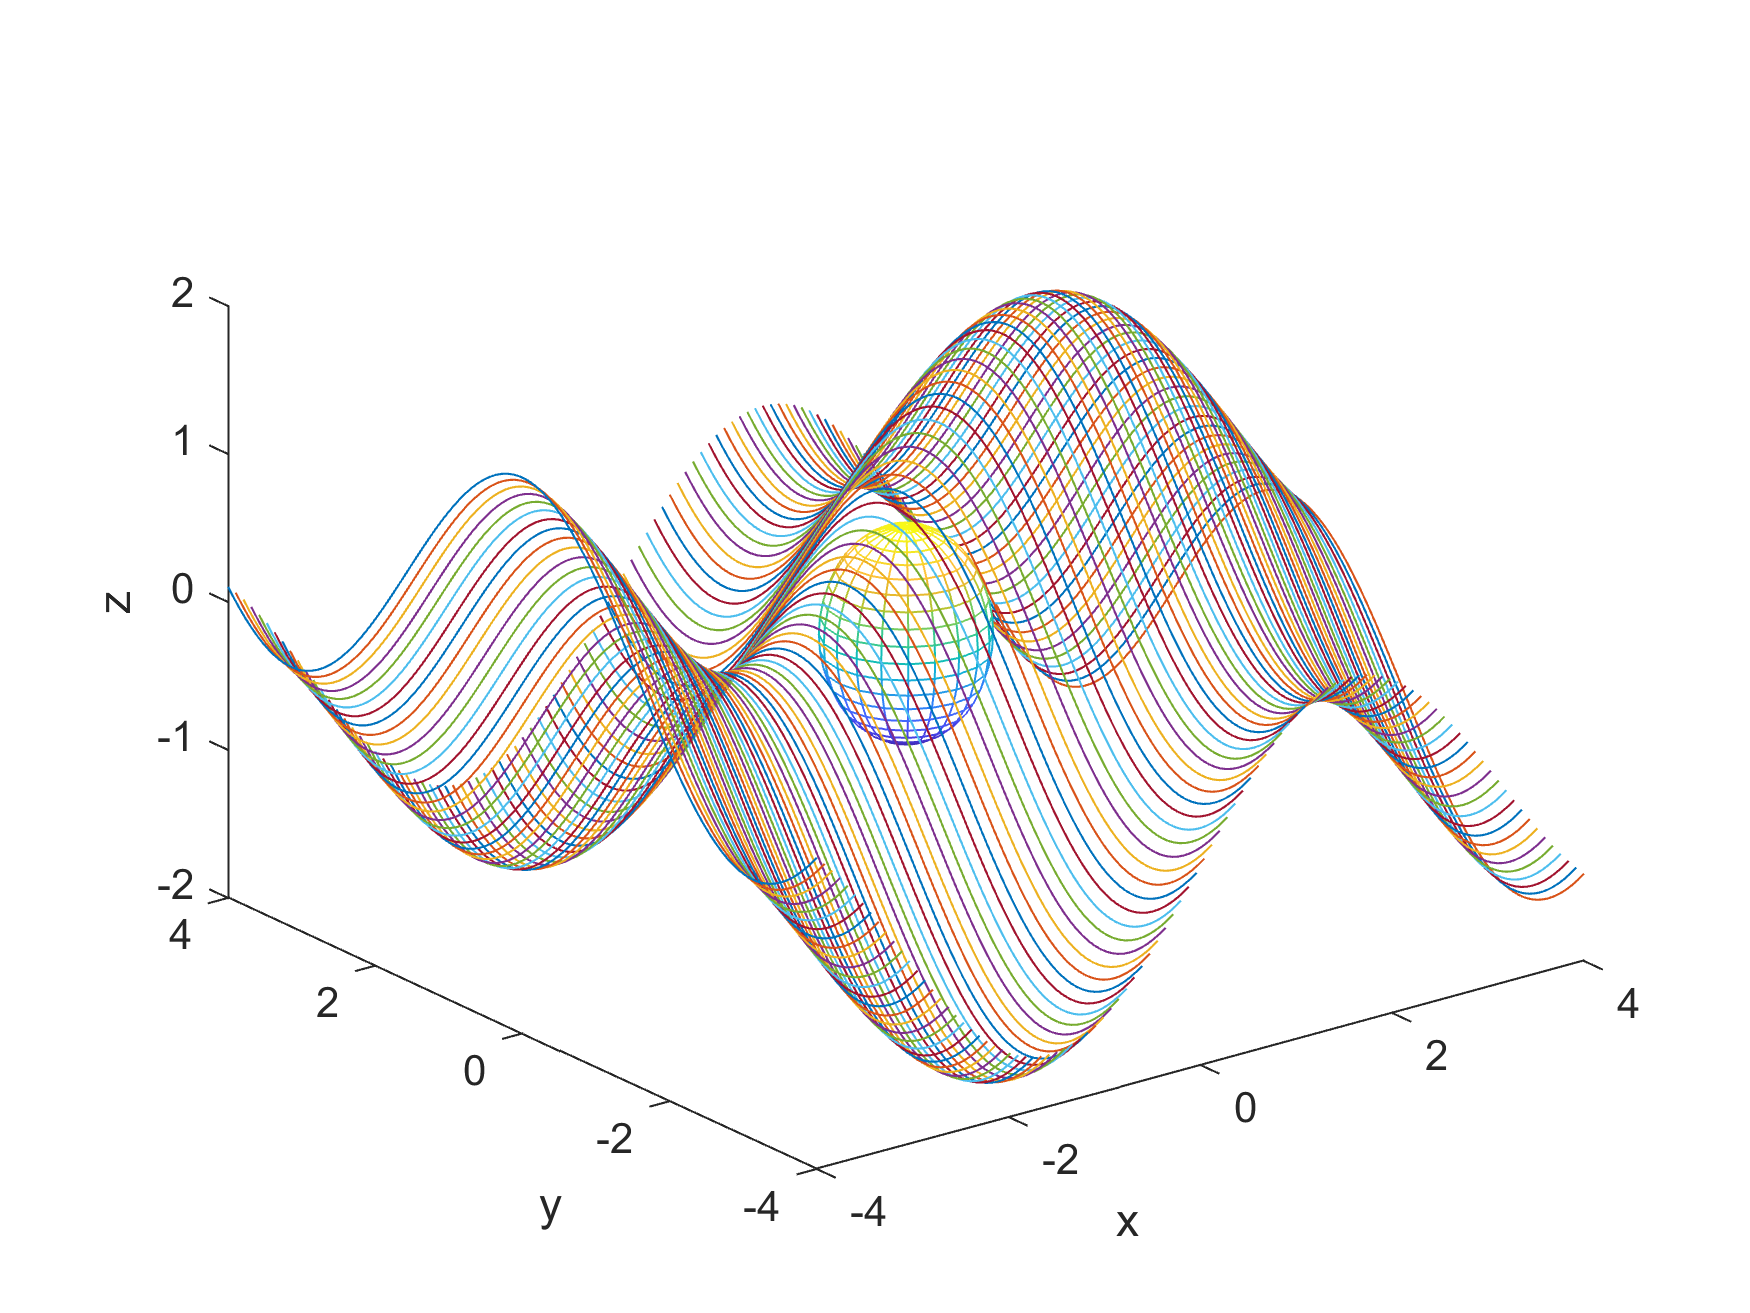
\includegraphics[width=12cm]{Q2/figures/plotwithSphere.png}
\end{figure}
\begin{figure}[H]
	\caption{Figure with Sphere Answer Another view}
	\centering
	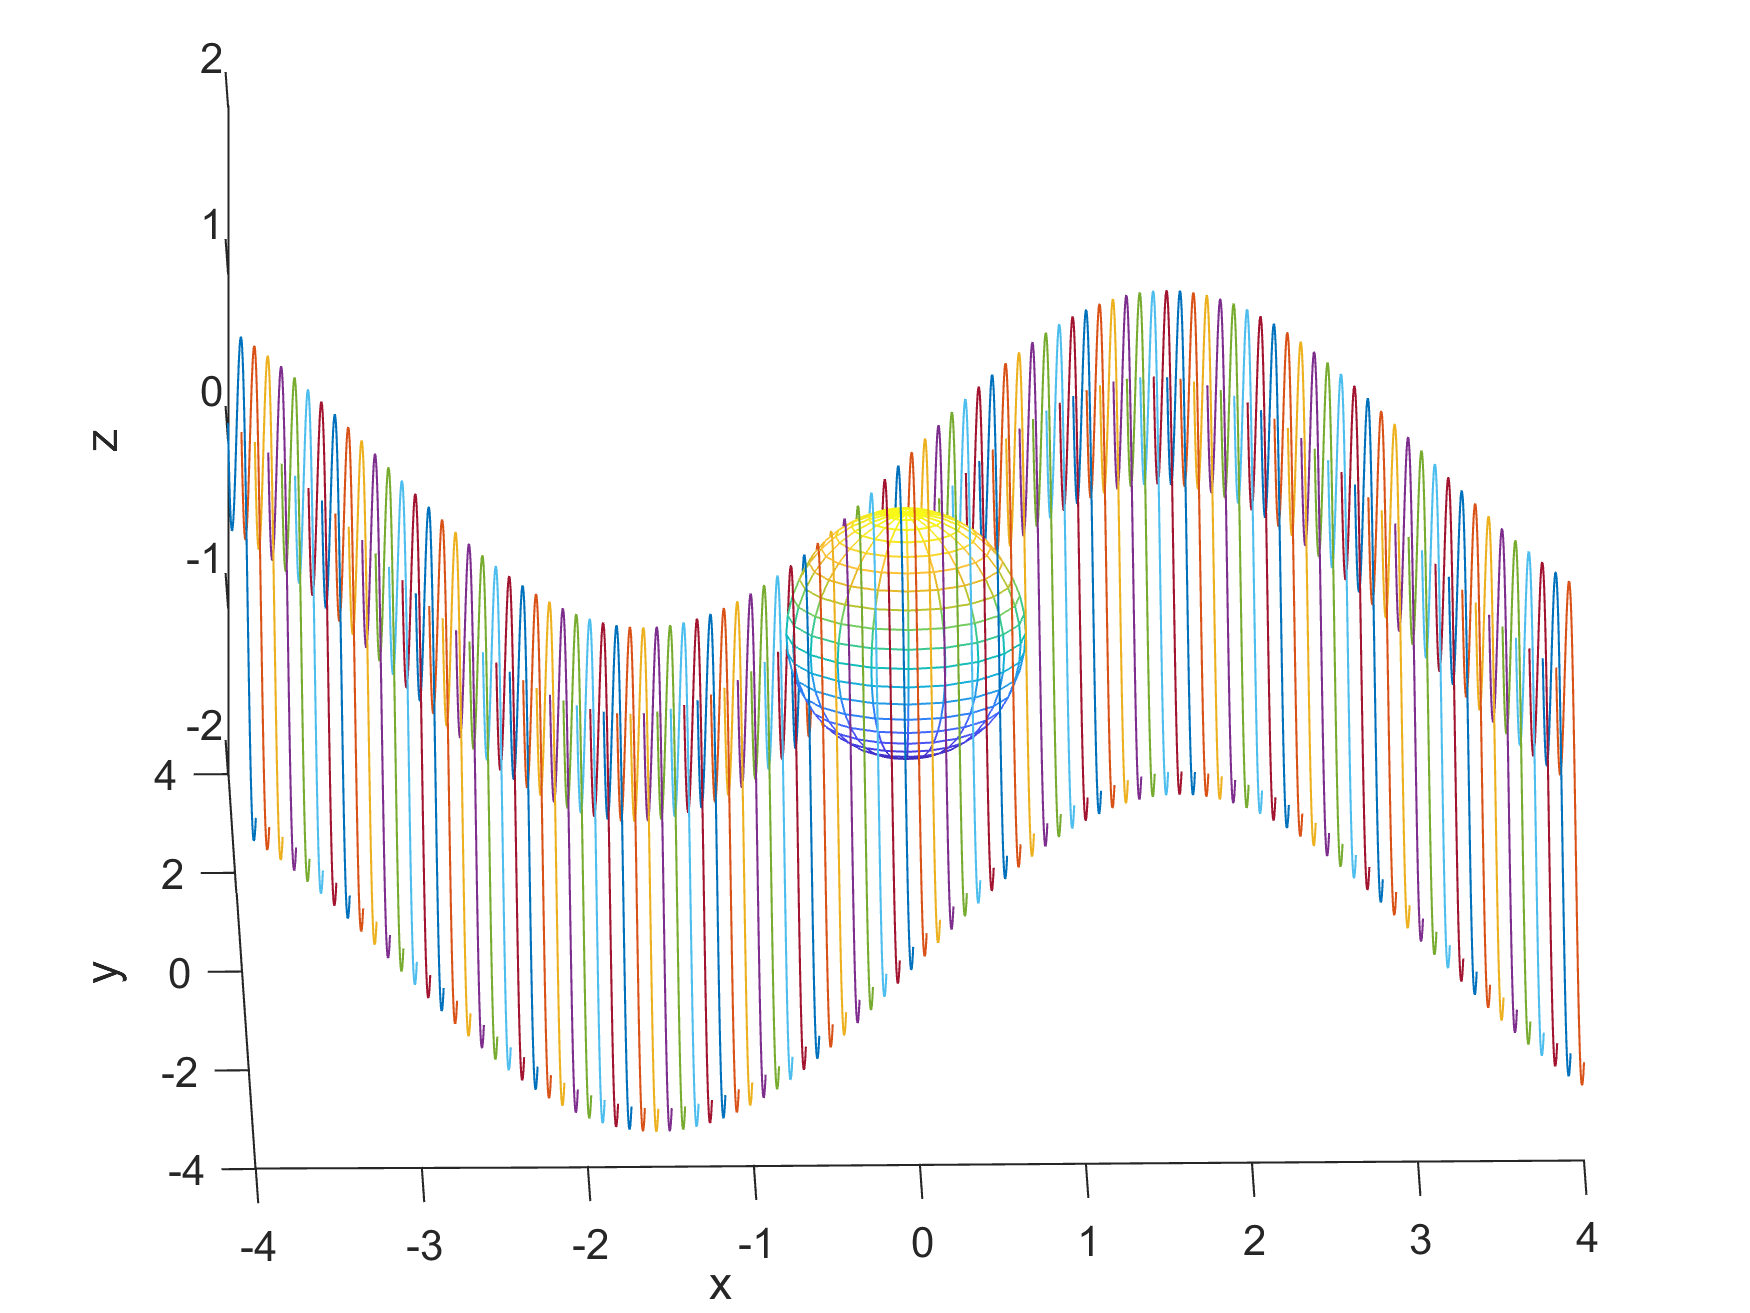
\includegraphics[width=12cm]{Q2/figures/plotwithSphereAnother.png}
\end{figure}